
	\section*{18/10}
	\begin{center}
		\textbf{Симплексный треугольный конечный элемент}
	\end{center}
	\[
	u=\alpha_1+\alpha_2 x +\alpha_3 y
	\]
	\begin{center}
	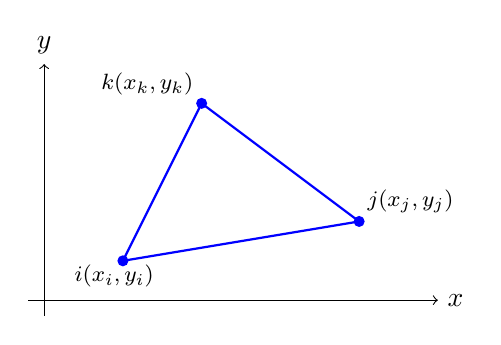
\begin{tikzpicture}
    		\draw[->] (-0.2,0) -- (5,0) node[right] {$x$};
    		\draw[->] (0,-0.2) -- (0,3) node[above] {$y$};
   		\draw[blue, thick] (1,0.5) -- (4,1) -- (2,2.5) -- cycle;
		{\footnotesize
   	 	\node at (1.5,0.55) [below left] {$i(x_i, y_i)$};
   		\node at (4,1) [above right] {$j(x_j, y_j)$};
    		\node at (2,2.5) [above left] {$k(x_k, y_k)$};
		}
		\fill[blue] (1, 0.5) circle (2pt);
		\fill[blue] (4,1) circle (2pt);
		\fill[blue] (2,2.5) circle (2pt);
	\end{tikzpicture}
	\end{center}
	\[
	\begin{cases}
		u_i=\alpha_1+\alpha_2 x_i +\alpha_3 y_i \\
		u_j=\alpha_1+\alpha_2 x_j +\alpha_3 y_j \\
		u_k=\alpha_1+\alpha_2 x_k +\alpha_3 y_k 
	\end{cases} \quad \Rightarrow \quad \Delta = \begin{vmatrix}
	1&x_i&y_i\\
	1&x_j&y_j\\
	1&x_k&y_k
	\end{vmatrix} = 2S_{\Delta}
	\]
	\[
	\Delta_1=\begin{vmatrix}
	u_i&x_i&y_i\\
	u_j&x_j&y_j\\
	u_k&x_k&y_k
	\end{vmatrix}
	 = u_i \underbrace{(x_jy_k-x_ky_j)}_{a_i} +u_j \underbrace{(x_ky_i-x_iy_k)}_{a_j}+u_k \underbrace{(x_iy_j-x_jy_i)}_{a_k}
	\]
	\[
	\Delta_2=\begin{vmatrix}
		1&u_i&y_i\\
		1&u_j&y_j\\
		1&u_k&y_k
	\end{vmatrix}
	= u_i \underbrace{(y_j-y_k)}_{b_i}+u_j \underbrace{(y_k-y_i)}_{b_j}+u_k \underbrace{(y_i-y_j)}_{b_k}
	\]
	\[
	\Delta_2=\begin{vmatrix}
		1&x_i&u_i\\
		1&x_j&u_j\\
		1&x_k&u_k
	\end{vmatrix}
	= u_i \underbrace{(x_k-x_j)}_{c_i}+u_j \underbrace{(x_i-x_k)}_{c_j}+u_k \underbrace{(x_j-x_i)}_{c_k}
	\]
	\[
	\alpha_1 = \frac{\Delta_1}{\Delta}, \quad \alpha_2 = \frac{\Delta_2}{\Delta}, \quad \alpha_3 = \frac{\Delta_3}{\Delta}
	\]
	\[
	u=\frac{1}{\Delta}(a_iu_i+a_ju_j+a_ku_k+b_iu_ix+b_ju_jx+b_ku_kx+c_iu_iy+c_ju_jy+c_ku_ky)=
	\]
	\[
	=\frac{1}{\Delta}\left[(a_i+b_ix+c_iy)u_i+(a_j+b_jx+c_jy)u_j+(a_k+b_kx+c_ky)u_i)\right]=
	\]
	\[
	=N_iu_i+N_ju_j+N_ku_k=\left[N\right]\left\{\Phi\right\}
	\]
	\[\{\Phi\} = [u_i, \ u_j,\ u_k]^T,\quad [N] = [N_i, \ N_j,\ N_k]\]
	\[
	\begin{cases}
		N_i = \frac{1}{\Delta}(a_i+b_ix+c_iy) \\
		N_j = \frac{1}{\Delta}(a_j+b_jx+c_jy) \\
		N_k = \frac{1}{\Delta}(a_k+b_kx+c_ky) 
	\end{cases} - \text{ функции формы, } u=\left[N\right]\left\{\Phi\right\}
	\]
	
	Свойства функций формы:
	\[\begin{cases}
	N_i(x_i, y_i) = 1,\ \ N_i(x_j, y_j) = 0,\ \ N_i(x_k, y_k) = 0;\\
	N_j(x_i, y_i) = 0,\ \ N_j(x_j, y_j) = 1,\ \ N_j(x_k, y_k) = 0;\\
	N_k(x_i, y_i) = 0,\ \ N_k(x_j, y_j) = 0,\ \ N_k(x_k, y_k) = 1;\\
	N_i + N_j + N_k = 1
	\end{cases}\]
	
	Возвращаемся к уравнению:
	\[
	\iint\limits_{\Omega} \left(\frac{\partial v}{\partial x} \cdot K_x \cdot  \frac{\partial u}{\partial x} + \frac{\partial v}{\partial y} \cdot K_y \cdot  \frac{\partial u}{\partial y} + buv-fv \right)dxdy-\]
	\[-\int\limits_{\text{Г}} \left(K_x \cdot  \frac{\partial u}{\partial x} \cdot l_x + K_y \cdot  \frac{\partial u}{\partial y} \cdot l_y \right)v\ d\xi = 0
	\]
	\[
	v=N\delta\Phi, \quad \delta\Phi=\left[v_i, v_j, v_k\right]^T
	\]
	\[
	\begin{bmatrix}
		\dfrac{\partial u}{\partial x} \\ \\ \dfrac{\partial u}{\partial y} 
	\end{bmatrix} = \begin{bmatrix}
	\dfrac{\partial \left[N\right]}{\partial x} \\  \\ \dfrac{\partial \left[N\right] }{\partial y} 
	\end{bmatrix} \left\{\Phi\right\} = \begin{bmatrix}
	\dfrac{\partial N_i}{\partial x} & \dfrac{\partial N_j}{\partial x} & \dfrac{\partial N_k}{\partial x} \\ & & \\ \dfrac{\partial N_i}{\partial y} & \dfrac{\partial N_j}{\partial y} & \dfrac{\partial N_k}{\partial y}
	\end{bmatrix} \left\{\Phi\right\} = \dfrac{1}{\Delta} \begin{bmatrix}
	b_i & b_ j & b_k \\ c_i & c_j & c_k
	\end{bmatrix} \left\{\Phi\right\} = \left[B\right] \left\{\Phi\right\}
	\]
	\[
	\begin{bmatrix}
		\dfrac{\partial v}{\partial x} \\ \\	\dfrac{\partial v}{\partial y}
	\end{bmatrix} = \left[B\right] \left\{\delta\Phi\right\} \qquad D=\begin{bmatrix}
	K_x & 0 \\ 0 & K_y
	\end{bmatrix}
	\]
	\[
	\int\limits_{\Omega} \left(\frac{\partial v}{\partial x} \cdot K_x \cdot  \frac{\partial u}{\partial x} + \frac{\partial v}{\partial y} \cdot K_y \cdot  \frac{\partial u}{\partial y}\right)\ dxdy = \int\limits_{\Omega} (B\delta\Phi)^TDB\Phi\ dxdy=
	\] 
	\[
	=\left\{ \delta \Phi \right\}^T \int\limits_{\Omega} B^T D B \ dxdy \ \left\{ \Phi \right\}
	\]
	\[
	\int\limits_{\Omega}  buv \ dxdy = \int\limits_{\Omega}  (N\delta \Phi) ^ T bN \Phi \ dxdy = \left\{ \delta \Phi \right\}^T \int\limits_{\Omega} bN^T N \ dxdy \ \left\{ \Phi \right\}
	\]
	\[
	\int\limits_{\Omega}fv\ dxdy = \{\delta\Phi\}^T \int\limits_{\Omega}f \cdot N^T \ dx dy
	\]
	\[
	\int\limits_{\Gamma} \hat \sigma \cdot v\ d\xi = \{\delta \Phi\}^T \int\limits_{\Gamma} \hat \sigma N^T\ d\xi
	\]
	\[
	K = \int\limits_{\Omega}(B^T D B + b N^T N)\ dx dy;\quad P = \int\limits_{\Omega}fN^T\ dx dy + \int\limits_{\Gamma} \hat \sigma N^T\ d\xi
	\]
	\[
	\{\delta\Phi\}^T K \Phi = \{\delta\Phi\}^T P \Rightarrow K \Phi = P
	\]
	\[
		\int\limits_{\Omega} B^T D B \ dx dy = \int\limits_{\Omega} \frac{1}{\Delta} 
		\begin{bmatrix}
		b_i & c_i\\
		b_j & c_j\\
		b_k & c_k\\
		\end{bmatrix}
		\cdot
		\begin{bmatrix}
		K_x & 0\\
		0 & K_y\\
		\end{bmatrix}
		\cdot
		\begin{bmatrix}
		b_i & b_j & b_k\\
		c_i & c_j & c_k\\
		\end{bmatrix}
		\ dx dy = \smiley
	\]
	
	
	Считаем, что $K_x, K_y - \text{const}$:
	\[
	\smiley = \dfrac{S_1}{(2S_1)^2} \left[K_x \begin{pmatrix}
		b_ib_i & b_ib_j & b_ib_k \\
		b_ib_j & b_jb_j & b_jb_k \\
		b_ib_k & b_jb_k & b_kb_k \\
	\end{pmatrix}+ K_y \begin{pmatrix}
	c_ic_i & c_ic_j & c_ic_k \\
	c_ic_j & c_jc_j & c_jc_k \\
	c_ic_k & c_jc_k & c_kc_k \\
	\end{pmatrix} \right] 
	\]
	\[
	\int\limits_{\Omega} b N^T N\ dx dy = \int\limits_{\Omega} b \begin{bmatrix}
		N_i \\ N_j \\ N_k
		\end{bmatrix}
		\cdot
		\begin{bmatrix}
		N_i & N_j & N_k
		\end{bmatrix}
		\ dx dy = 
	\]
	\[
	= \int\limits_{\Omega} b \cdot
	\begin{bmatrix}
	N_iN_i & N_iN_j & N_iN_k \\
	N_iN_j & N_jN_j & N_jN_k \\
	N_iN_k & N_jN_k & N_kN_k \\
	\end{bmatrix}
	\ dx dy
	\]
	\[
	P_1 = \int\limits_{\Omega} f N^T \ dx dy = \int\limits_{\Omega} f \cdot 
	\begin{bmatrix}
		N_i \\ N_j \\ N_k
		\end{bmatrix}
	\ dx dy
	\]
	\newpage
	\begin{center}
		\textbf{Естественная система координат}
	\end{center}
	\begin{center}
	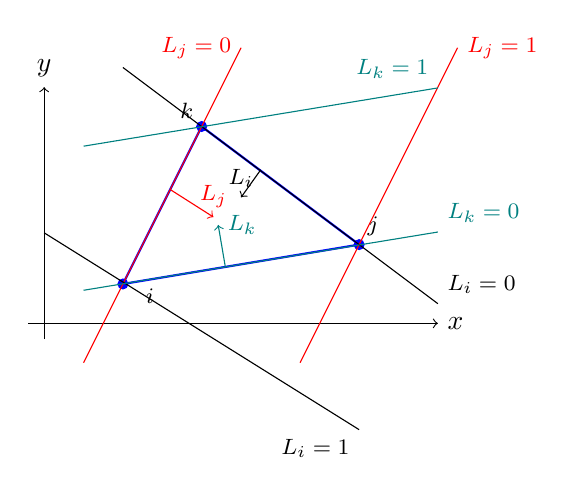
\begin{tikzpicture}
    		\draw[->] (-0.2,0) -- (5,0) node[right] {$x$};
    		\draw[->] (0,-0.2) -- (0,3) node[above] {$y$};
   		\draw[blue, thick] (1,0.5) -- (4,1) -- (2,2.5) -- cycle;
		{\footnotesize
   	 	\node at (1.5,0.55) [below left] {$i$};
   		\node at (4,1) [above right] {$j$};
    		\node at (2,2.5) [above left] {$k$};
		}
		\fill[blue] (1, 0.5) circle (2pt);
		\fill[blue] (4,1) circle (2pt);
		\fill[blue] (2,2.5) circle (2pt);
		
		\draw[thin, red] (0.5,-0.5) -- (2.5, 3.5) node[left] {\footnotesize $L_j = 0$};
		\draw[thin, red] (3.25,-0.5) -- (5.25, 3.5) node[right] {\footnotesize $L_j = 1$};
		
		\draw[thin] (1, 3.25) -- (5,0.25) node[above right] {\footnotesize $L_i = 0$};
		\draw[thin] (0, 1.15) -- (4,-1.35) node[below left] {\footnotesize $L_i = 1$};
		
		\draw[thin, teal] (0.5, 0.42) -- (5, 1.16) node[above right] {\footnotesize $L_k = 0$};
		\draw[thin, teal] (0.5, 2.25) -- (5, 2.99) node[above left] {\footnotesize $L_k = 1$};
		
		\draw[->][thin, teal] (2.3, 0.72) -- (2.21,1.25) node[right] {\footnotesize $L_k$};
		\draw[->][thin, red] (1.6, 1.7) -- (2.15,1.35) node[above] {\footnotesize $L_j$};
		\draw[->][thin] (2.75, 1.95) -- (2.5,1.6) node[above] {\footnotesize $L_i$};
	\end{tikzpicture}
	\end{center}
	\[\begin{cases}
	0 \leq L_i \leq 1;\\
	0 \leq L_j \leq 1;\\
	0 \leq L_k \leq 1.
	\end{cases}\]

	\begin{minipage}{0.45\textwidth}
	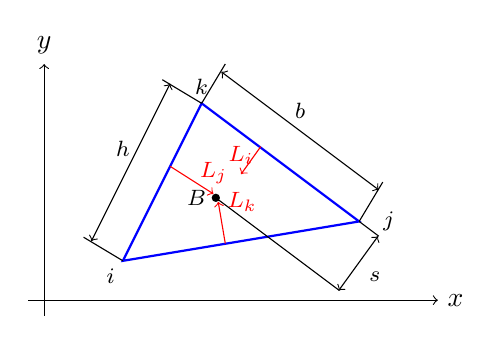
\begin{tikzpicture}
    		\draw[->] (-0.2,0) -- (5,0) node[right] {$x$};
    		\draw[->] (0,-0.2) -- (0,3) node[above] {$y$};
   		\draw[blue, thick] (1,0.5) -- (4,1) -- (2,2.5) -- cycle;
		{\footnotesize
   	 	\node at (1,0.5) [below left] {$i$};
   		\node at (4.2,1) [right] {$j$};
    		\node at (2,2.5) [above] {$k$};
		}
		
		\draw[->][thin, red] (2.3, 0.72) -- (2.21,1.25) node[right] {\footnotesize $L_k$};
		\draw[->][thin, red] (1.6, 1.7) -- (2.15,1.35) node[above] {\footnotesize $L_j$};
		\draw[->][thin, red] (2.75, 1.95) -- (2.5,1.6) node[above] {\footnotesize $L_i$};
		
		\fill (2.18,1.3) circle (1.5pt) node[left] {\footnotesize$B$};
		
		\draw (4,1) -- (4.25, 0.8125);
		\draw (2.18,1.3) -- (3.75, 0.1225);
		\draw[<->] (4.24, 0.8126) -- (3.74, 0.1226);
		\node at (4.2, 0.3) {\footnotesize$s$};
		
		\draw (2,2.5) -- (2.3, 3);
		\draw (4,1) -- (4.3, 1.5);
		\draw[<->] (2.25, 2.9) -- (4.25, 1.4);
		\node at (3.25, 2.4) {\footnotesize$b$};
		
		\draw (2,2.5) -- (1.5, 2.8);
		\draw (1,0.5) -- (0.5, 0.8);
		\draw[<->] (1.6, 2.75) -- (0.6, 0.75);
		\node at (1, 1.92) {\footnotesize$h$};
	\end{tikzpicture}
\end{minipage}
\hfill
\begin{minipage}{0.45\textwidth}
	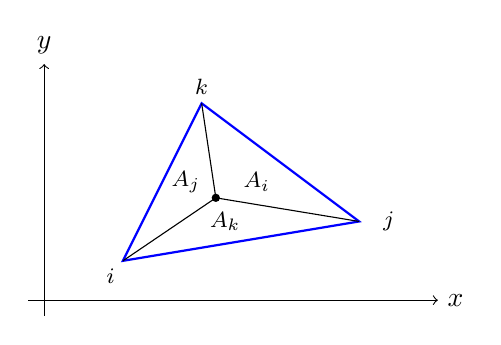
\begin{tikzpicture}
    		\draw[->] (-0.2,0) -- (5,0) node[right] {$x$};
    		\draw[->] (0,-0.2) -- (0,3) node[above] {$y$};
   		\draw[blue, thick] (1,0.5) -- (4,1) -- (2,2.5) -- cycle;
		{\footnotesize
   	 	\node at (1,0.5) [below left] {$i$};
   		\node at (4.2,1) [right] {$j$};
    		\node at (2,2.5) [above] {$k$};
		}
		
		\fill (2.18,1.3) circle (1.5pt);
		
		\draw (1,0.5) -- (2.18,1.3);
		\draw (4,1) -- (2.18,1.3);
		\draw (2,2.5) -- (2.18,1.3);
		
		\node at (2.7, 1.5) {\footnotesize$A_i$};
		\node at (1.8, 1.5) {\footnotesize$A_j$};
		\node at (2.3, 1) {\footnotesize$A_k$};

	\end{tikzpicture}
\end{minipage}
\[\begin{cases}
S_{\triangle} = \frac{1}{2} bh,\\
S_{A_i} =  \frac{1}{2} bs
\end{cases}
\Rightarrow
L_i = \frac{S_{A_i}}{S_{\triangle}} = \frac{s}{h}
\]
\[L_j = \frac{S_{A_j}}{S_{\triangle}},\ \ L_k = \frac{S_{A_k}}{S_{\triangle}}\]
\[L_i + L_j + L_k = \frac{S_{A_i} + S_{A_j} + S_{A_k}}{S_{\triangle}} = 1\]
\[N_i = L_i,\ N_j = L_j,\ N_k = L_k\]